\documentclass[unicode,11pt,a4paper,oneside,numbers=endperiod,openany]{scrartcl}
\usepackage{graphicx}
\usepackage{subfig}
\usepackage{float}

\usepackage{ifthen}
\usepackage[utf8]{inputenc}
\usepackage{graphics}
\usepackage{graphicx}
\usepackage{hyperref}

\pagestyle{plain}
\voffset -5mm
\oddsidemargin  0mm
\evensidemargin -11mm
\marginparwidth 2cm
\marginparsep 0pt
\topmargin 0mm
\headheight 0pt
\headsep 0pt
\topskip 0pt        
\textheight 255mm
\textwidth 165mm

\newcommand{\duedate} {}
\newcommand{\setduedate}[1]{%
\renewcommand\duedate {Due date:~ #1}}
\newcommand\isassignment {false}
\newcommand{\setassignment}{\renewcommand\isassignment {true}}
\newcommand{\ifassignment}[1]{\ifthenelse{\boolean{\isassignment}}{#1}{}}
\newcommand{\ifnotassignment}[1]{\ifthenelse{\boolean{\isassignment}}{}{#1}}

\newcommand{\assignmentpolicy}{
\begin{table}[h]
\begin{center}
\scalebox{0.8} {%
\begin{tabular}{|p{0.02cm}p{16cm}|}
\hline
&\\
\multicolumn{2}{|c|}{\Large\textbf{HPC  2022 ---  Submission Instructions}}\\
\multicolumn{2}{|c|}{\large\textbf{(Please, notice that following instructions are mandatory: }}\\
\multicolumn{2}{|c|}{\large\textbf{submissions that don't comply with, won't be considered)}}\\
&\\
\textbullet & Assignments must be submitted to \href{https://www.icorsi.ch/course/view.php?id=14652}{iCorsi} (i.e. in electronic format).\\
\textbullet & Provide both executable package and sources (e.g. C/C++ files, Matlab). 
If you are using libraries, please add them in the file. Sources must be organized in directories called:\\
\multicolumn{2}{|c|}{\textit{Project\_number\_lastname\_firstname}}\\
& and  the  file must be called:\\
\multicolumn{2}{|c|}{\textit{project\_number\_lastname\_firstname.zip}}\\
\multicolumn{2}{|c|}{\textit{project\_number\_lastname\_firstname.pdf}}\\
\textbullet &  The TAs will grade your project by reviewing your project write-up, and looking at the implementation 
                 you attempted, and benchmarking your code's performance.\\

\textbullet & You are allowed to discuss all questions with anyone you like; however: (i) your submission must list anyone you discussed problems with and (ii) you must write up your submission independently.\\
\hline
\end{tabular}
}
\end{center}
\end{table}
}
\newcommand{\punkte}[1]{\hspace{1ex}\emph{\mdseries\hfill(#1~\ifcase#1{Points}\or{Points}\else{Points}\fi)}}


\newcommand\serieheader[6]{
\thispagestyle{empty}%
\begin{flushleft}

\includegraphics[width=0.4\textwidth]{usi_inf.png}
\end{flushleft}
  \noindent%
  {\large\ignorespaces{\textbf{#1}}\hspace{\fill}\ignorespaces{ \textbf{#2}}}\\ \\%
  {\large\ignorespaces #3 \hspace{\fill}\ignorespaces #4}\\
  \noindent%
  \bigskip
  \hrule\par\bigskip\noindent%
  \bigskip {\ignorespaces {\Large{\textbf{#5}}}
  \hspace{\fill}\ignorespaces \large \ifthenelse{\boolean{\isassignment}}{\duedate}{#6}}
  \hrule\par\bigskip\noindent%  \linebreak
 }

\makeatletter
\def\enumerateMod{\ifnum \@enumdepth >3 \@toodeep\else
      \advance\@enumdepth \@ne
      \edef\@enumctr{enum\romannumeral\the\@enumdepth}\list
      {\csname label\@enumctr\endcsname}{\usecounter
        {\@enumctr}%%%? the following differs from "enumerate"
	\topsep0pt%
	\partopsep0pt%
	\itemsep0pt%
	\def\makelabel##1{\hss\llap{##1}}}\fi}
\let\endenumerateMod =\endlist
\makeatother




\usepackage{textcomp}





\begin{document}


\setassignment
\setduedate{02.11.2022, 23:59}

\serieheader{High-Performance Computing}{2022}{Student: SIMONE TARENZI}{Discussed with: FULL NAME}{Solution for Project 3}{}
\newline

\section{Task: Implementing the linear algebra functions and the stencil operators [35 Points]}

Nothing really interesting to be said about implementing the hpc functions and stencil operators.
\newline
\begin{figure}[H]
\centering
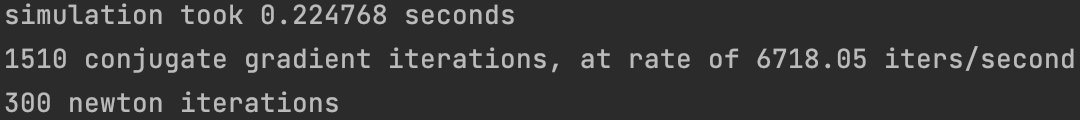
\includegraphics[width=0.7\linewidth]{terminal128.png}
\caption{the output of the terminal for the 128x128 grid}
\end{figure}

\begin{figure}[H]
\centering
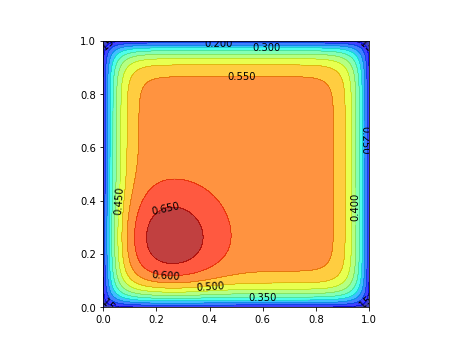
\includegraphics[width=0.7\linewidth]{output128.png}
\caption{the output.png file of the 128x128 grid created by plotting.py}
\end{figure}

I've also tried doing a test with a 500x500 grid size.
\begin{figure}[H]
\centering
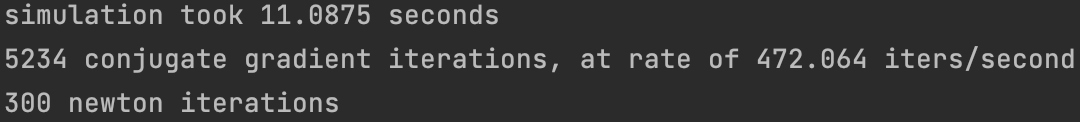
\includegraphics[width=0.7\linewidth]{terminal500.png}
\caption{the output of the terminal for the 500x500 grid}
\end{figure}
\begin{figure}[H]
\centering
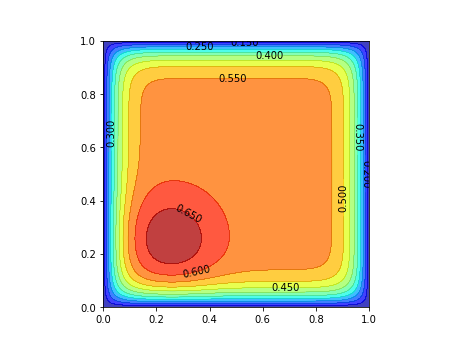
\includegraphics[width=0.7\linewidth]{output500.png}
\caption{the output.png file of the 500x500 grid created by plotting.py}
\end{figure}


\section{Task:  Adding OpenMP to the nonlinear PDE mini-app [50 Points]}

First of all I've added the int numThreads in the data header that can be set directly by calling the main from the terminal. This makes it way easier to run and plot the result of the program using a varying number of OpenMP threads.
\newline
After that, implementing the parallel versions of the hpc\_xxxx() functions was very straightforward. 
\newline
Using 4 threads showed great results for both the 128 and 256 grids, but the 512 had its best ones while using 16 threads.
\newline
\begin{figure}[H]
\centering
  \subfloat[Using 1 thread on a 128x128 grid]{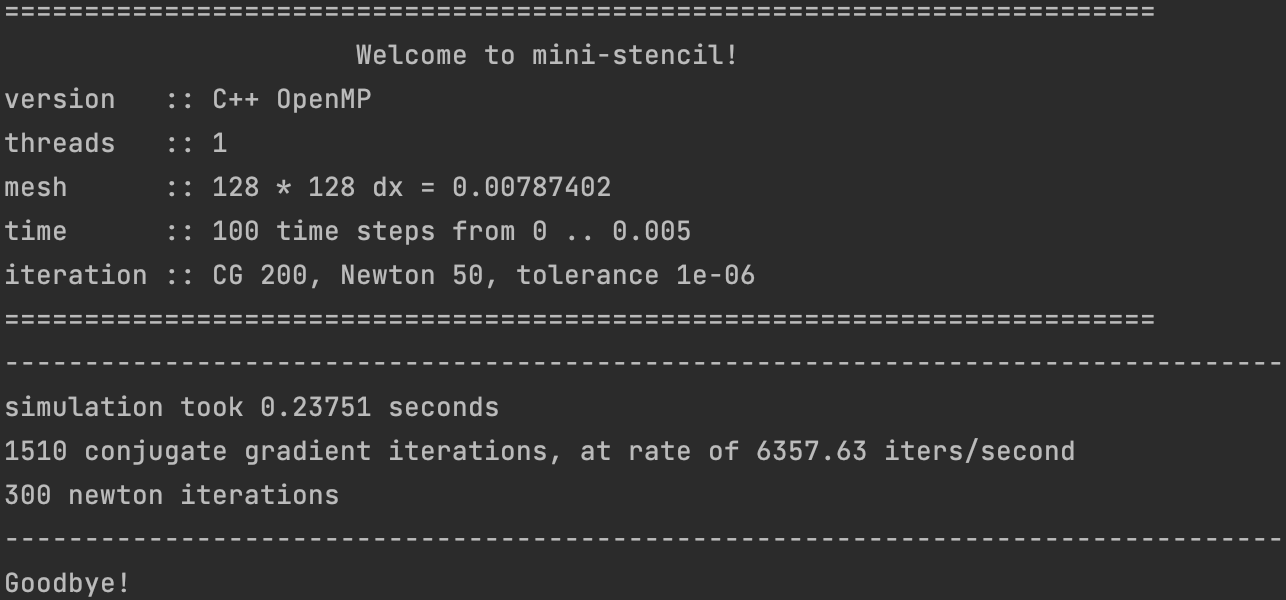
\includegraphics[width=0.49\textwidth]{terminal1x128.png}\label{fig:f1}}
  \hfill
  \subfloat[Using 4 threads on a 128x128 grid]{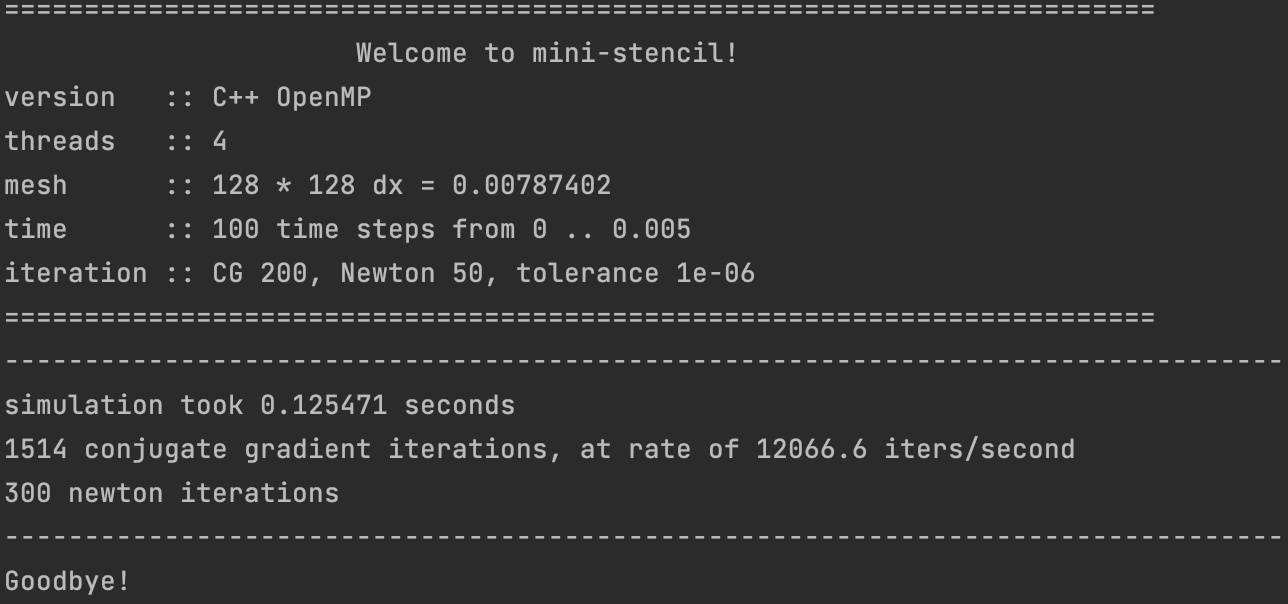
\includegraphics[width=0.49\textwidth]{terminal4x128.png}\label{fig:f2}}
  \caption{comparison between two runs of the program on a 128x128 grid with 1 and 4 threads}
\end{figure}
\begin{figure}[H]
\centering
  \subfloat[Using 1 thread on a 256x256 grid]{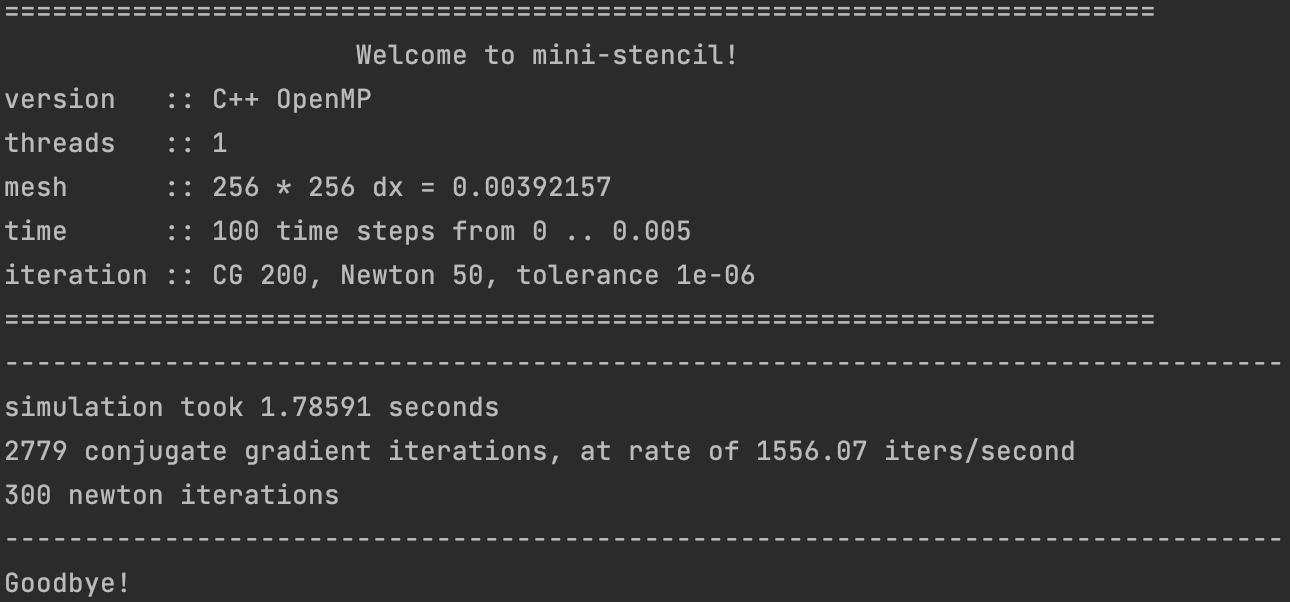
\includegraphics[width=0.49\textwidth]{terminal1x256.png}\label{fig:f1}}
  \hfill
  \subfloat[Using 4 threads on a 256x256 grid]{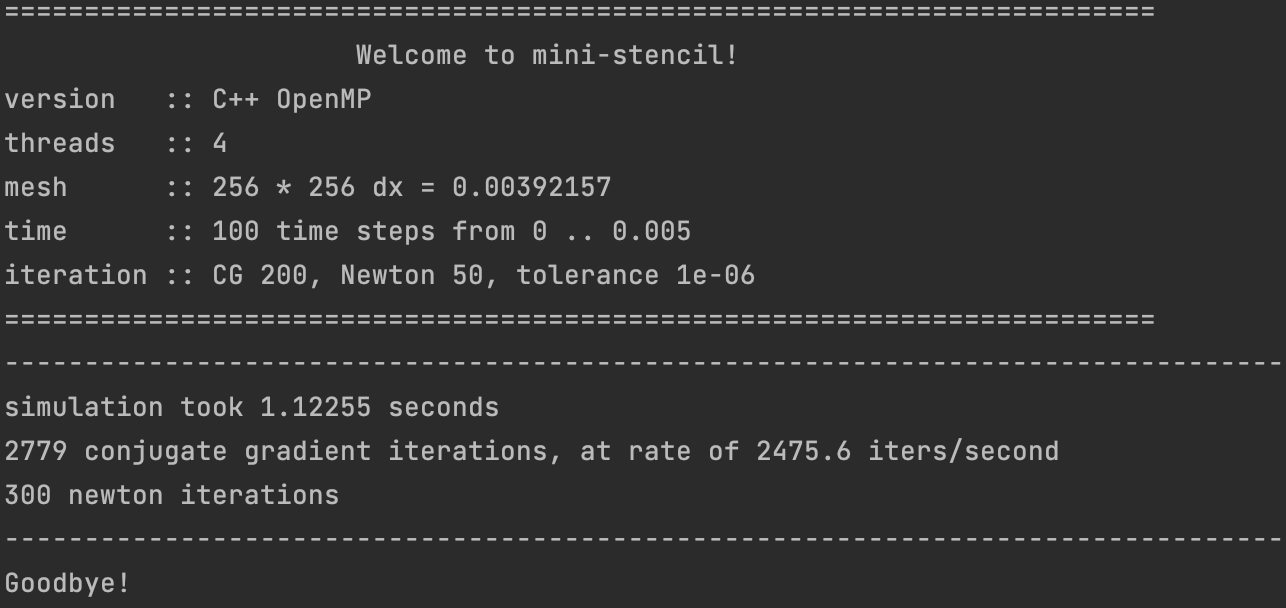
\includegraphics[width=0.49\textwidth]{terminal4x256.png}\label{fig:f2}}
  \caption{comparison between two runs of the program on a 256x256 grid with 1 and 4 threads}
\end{figure}
\begin{figure}[H]
\centering
  \subfloat[Using 4 threads on a 512x512 grid]{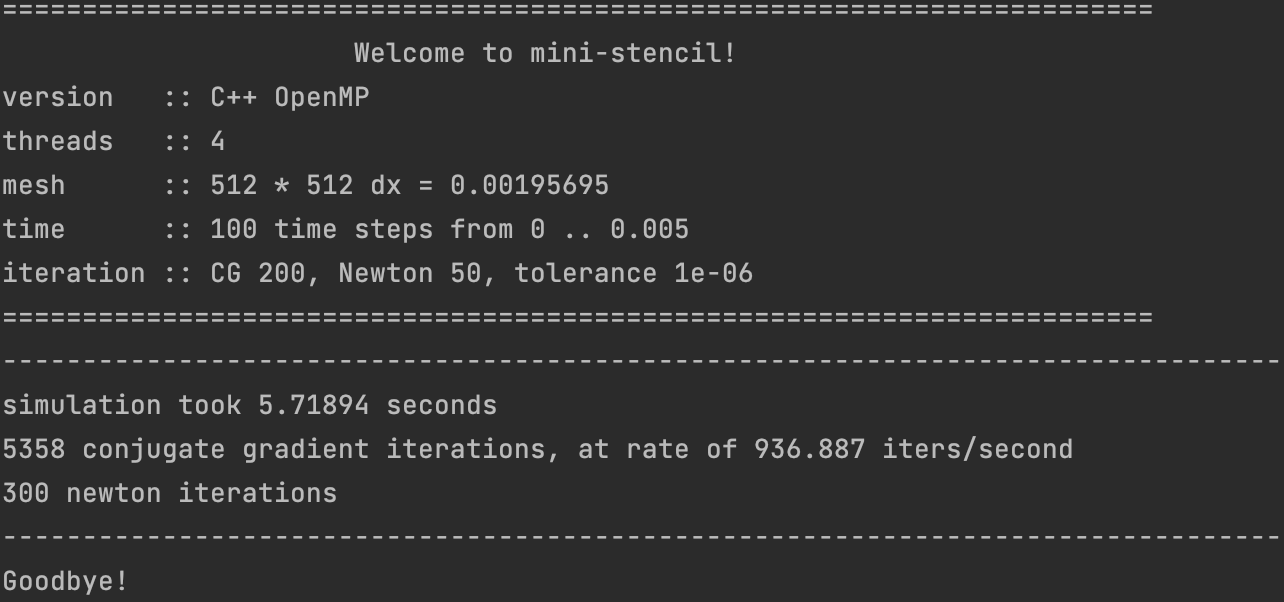
\includegraphics[width=0.49\textwidth]{terminal4x512.png}\label{fig:f1}}
  \hfill
  \subfloat[Using 16 threads on a 512x512 grid]{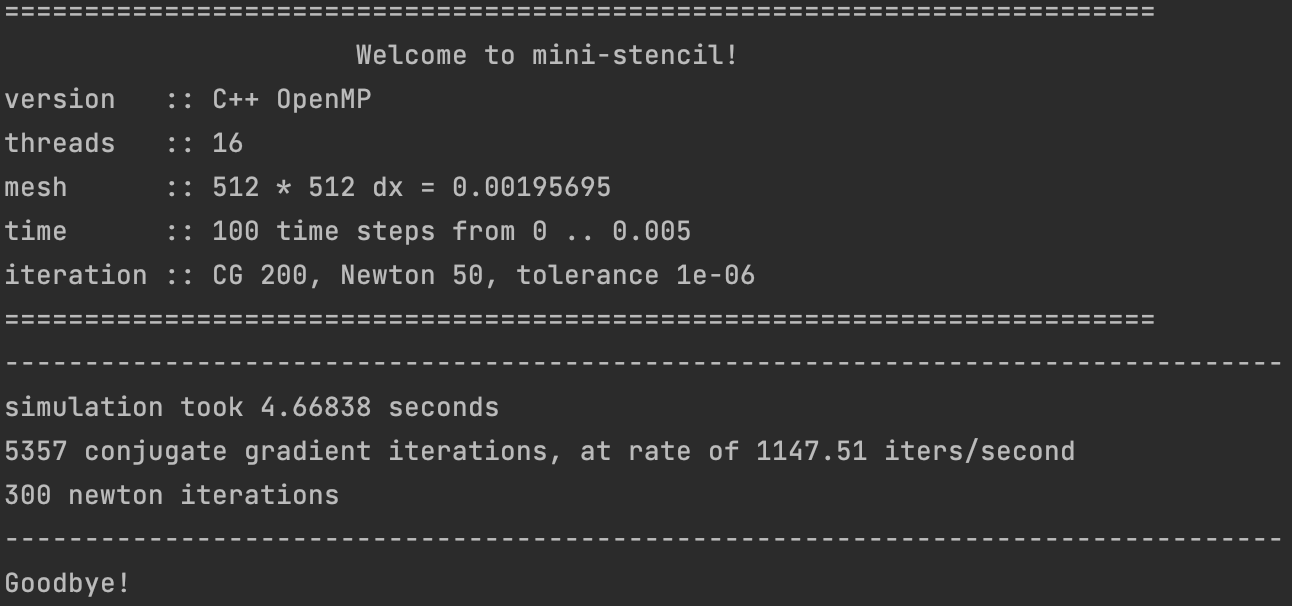
\includegraphics[width=0.49\textwidth]{terminal16x512.png}\label{fig:f2}}
  \caption{comparison between two runs of the program on a 512x512 grid with 4 and 16 threads}
\end{figure}
Next, the exercise asked to implement the parallelization for the stencil operators of the grid and plot the performance of various grid sizes while using a number of threads going from 1 to 24.
\newline
First I implemented parallelization for the interior grid points and the inner east, west, north and south boundaries.
\newline
Then I created a manual\_plot.py file that shows the performance for the various thread numbers.
\newline
I also modified the main class so that it writes to a txt file the time taken for the program to run.
\newline
Being the first time I used Python, I simply copy-pasted the results in the manual\_plot.py file.
\newline
\begin{figure}[H]
\centering
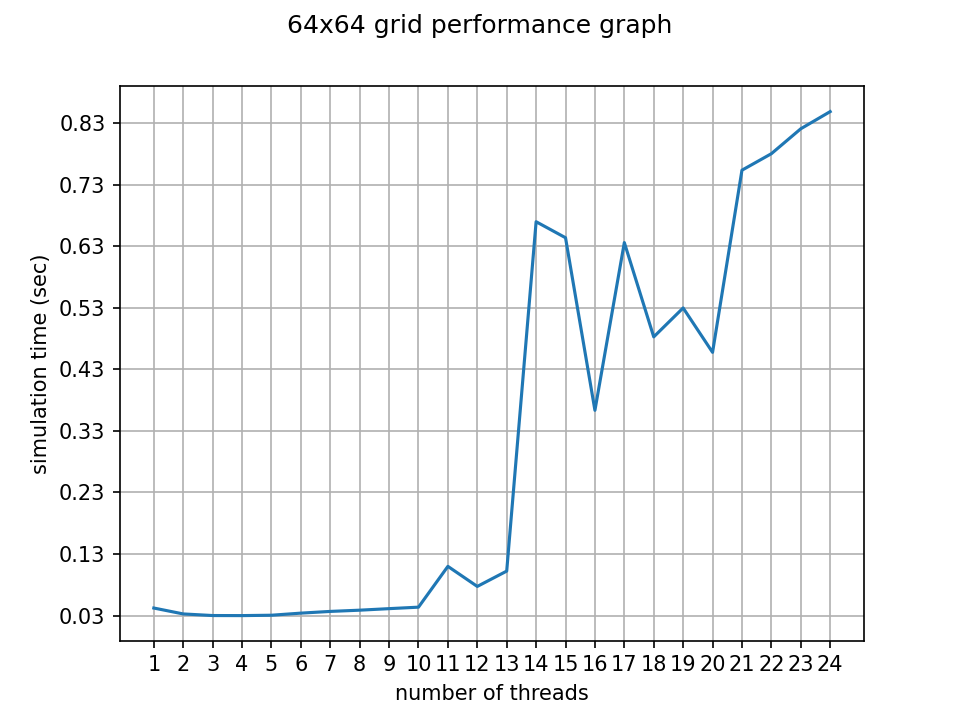
\includegraphics[width=0.8\linewidth]{64manualplot.png}
\caption{performance of the parallel version of the program for a 64x64 grid}
\end{figure}
\begin{figure}[H]
\centering
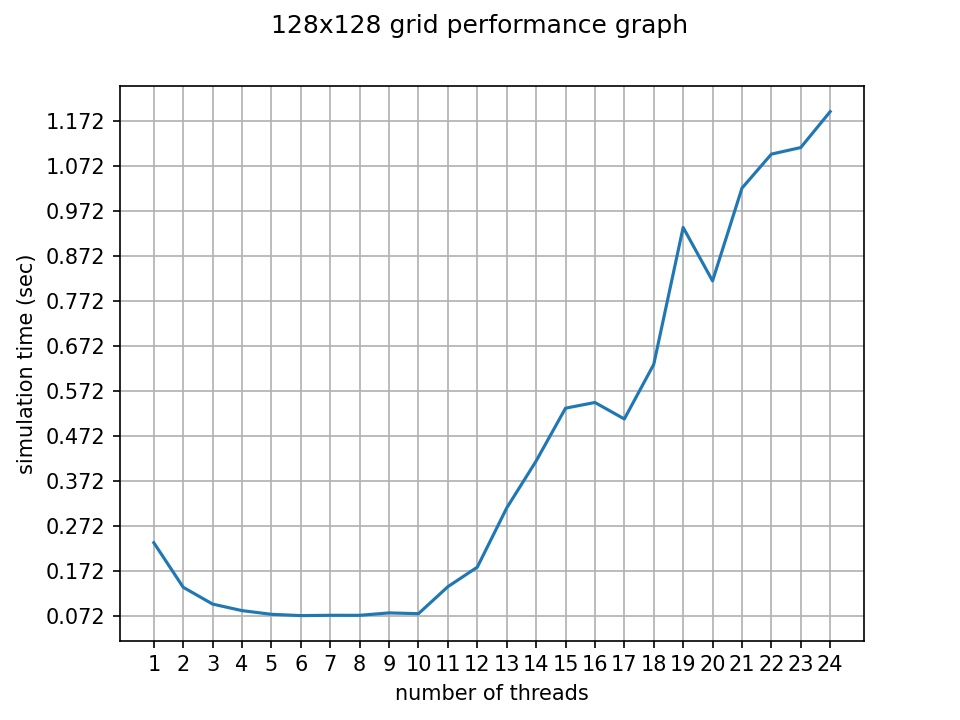
\includegraphics[width=0.8\linewidth]{128manualplot.png}
\caption{performance of the parallel version of the program for a 128x128 grid}
\end{figure}
\begin{figure}[H]
\centering
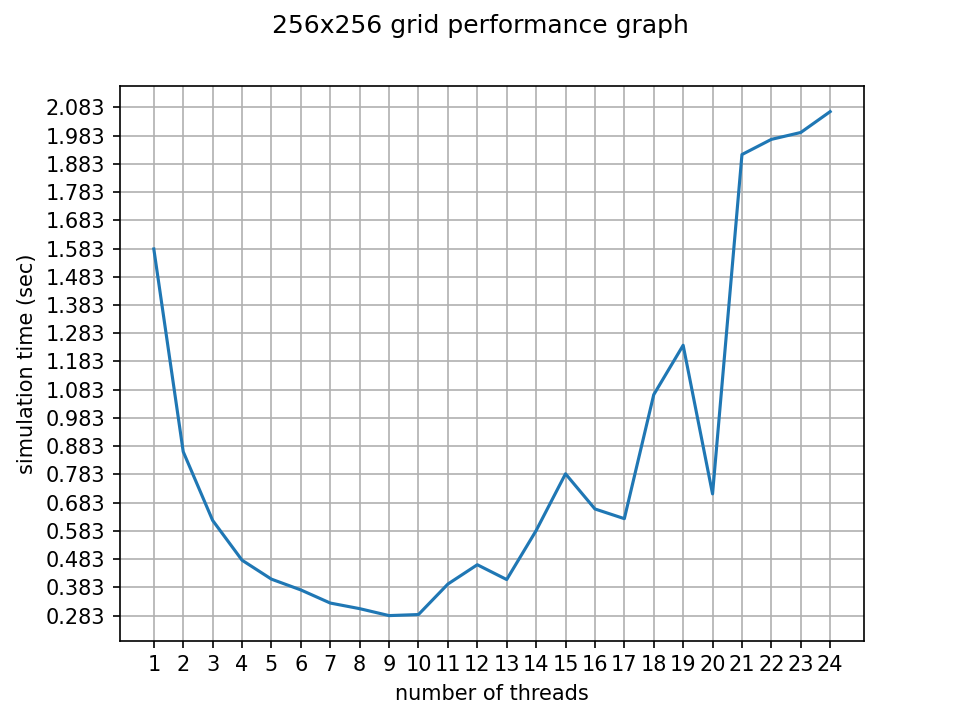
\includegraphics[width=0.8\linewidth]{256manualplot.png}
\caption{performance of the parallel version of the program for a 256x256 grid}
\end{figure}
\begin{figure}[H]
\centering
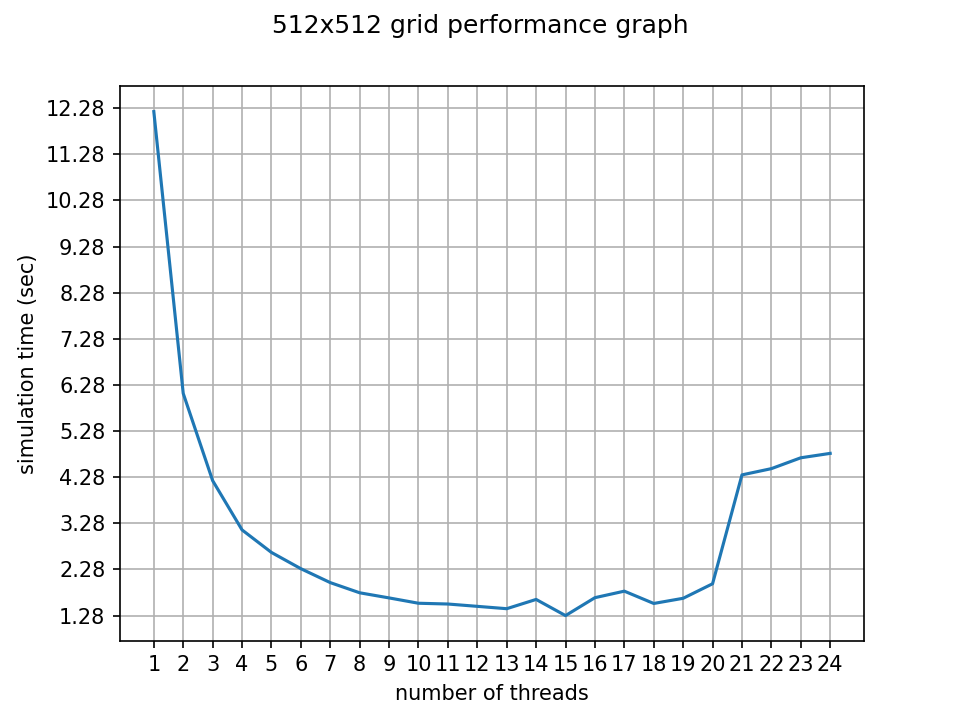
\includegraphics[width=0.8\linewidth]{512manualplot.png}
\caption{performance of the parallel version of the program for a 512x512 grid}
\end{figure}
\begin{figure}[H]
\centering
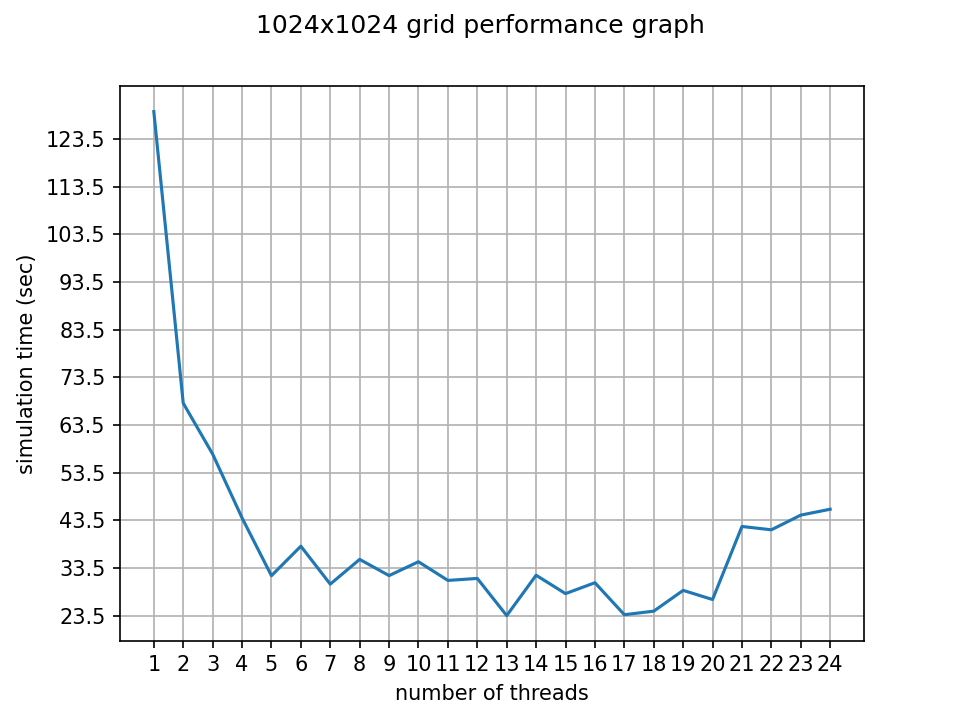
\includegraphics[width=0.8\linewidth]{1024manualplot.png}
\caption{performance of the parallel version of the program for a 1024x1024 grid}
\end{figure}

The 64x64 grid clearly shows the better results when using a small number of threads: in particular, using 4 threads consistently demonstrates the best performance, getting progressively worse when increasing the number of threads.


\section{Task:  Quality of the Report  [15 Points]}



\end{document}